
The previous Section \ref{sec:experiments} looked at the performance of the different naming models using vanilla evaluation methods like accuracy.
This way of evaluating object naming is unsatisfactory: the ManyNames data, and also our verification data, clearly shows that human annotators often agree on a certain entry-level name with other names might be adequate too.
In the following, we show how our verification data can be used to gain more detailed insights into the way different naming models calibrate their decisions and reflect human-like naming behaviour.

\begin{table*}[t]
\centering
	\small
\begin{tabular}{ll||rr|rrr}
\toprule
&  & \multicolumn{2}{c|}{Correct} & \multicolumn{3}{c}{Incorrect}\\
                         model &  gt &  hit &  valid &  human-like &  related &  off \\
\midrule
       FRCNN$_{\text{VG1600}}$ &  VG & 74.8 &     13.7 &         5.3 &      1.7 &    4.5 \\
        FRCNN$_{\text{MN442}}$ &  VG & 71.1 &     13.6 &         5.3 &      2.6 &    7.4 \\
        \midrule
 FRCNN$_{\text{VG1600--VGMN}}$ &  MN & 80.7 &      9.0 &         3.7 &      3.4 &    3.3 \\
         \midrule
     ResNet101$_{\text{VGMN}}$ &  VG & 62.8 &     11.6 &         5.2 &     10.3 &   10.1 \\
     ResNet101$_{\text{VGMN}}$ &  MN & 68.7 &      9.9 &         5.5 &      7.7 &    8.2 \\
    ResNet101$_{\text{MN442}}$ &  MN & 69.7 &      9.9 &         5.9 &      7.0 &    7.6 \\
    ResNet101$_{\text{MN442}}$ &  VG & 63.8 &     11.9 &         5.7 &      8.8 &    9.9 \\
\bottomrule
\end{tabular}


\caption{Model results for different categories of errors} \label{tab:humanlike}
\end{table*}


\begin{table*}[t]
\centering
	\small
\begin{tabular}{ll|rrr|rrr}
\toprule
&  & \multicolumn{3}{c|}{MN agreement $>$ 0.9} & \multicolumn{3}{c}{MN agreement $\leq$0.9}\\
                         model &  gt &  hit &  valid &  incorrect &  hit &  valid &  incorrect \\
\midrule
       FRCNN$_{\text{VG1600}}$ &  VG &   94.8 &      0.8 &      4.4 &   63.6 &     21.0 &     15.5 \\
        FRCNN$_{\text{MN442}}$ &  VG &   89.6 &      0.8 &      9.6 &   60.7 &     20.8 &     18.5 \\
                \midrule
 FRCNN$_{\text{VG1600--VGMN}}$ &  MN &   94.5 &      0.0 &      5.5 &   72.9 &     14.0 &     13.1 \\
         \midrule
     ResNet101$_{\text{VGMN}}$ &  VG &   88.3 &      0.5 &     11.2 &   48.5 &     17.8 &     33.7 \\
     ResNet101$_{\text{VGMN}}$ &  MN &   89.6 &      0.5 &      9.9 &   57.0 &     15.2 &     27.8 \\
    ResNet101$_{\text{MN442}}$ &  MN &   90.1 &      0.5 &      9.4 &   58.2 &     15.2 &     26.7 \\
    ResNet101$_{\text{MN442}}$ &  VG &   88.6 &      0.8 &     10.6 &   49.9 &     18.1 &     32.1 \\
\bottomrule
\end{tabular}
\caption{Break-down of the results (in \%) according to the agreement level of the MN name: Categorization of a predicted name\ $\hat{n}$ into either a \textit{hit}, \textit{correct} (less preferred name, synonym, hypernym/hyponym), or \textit{wrong} \label{tab:exp_errors_agreement}}
\end{table*}

\paragraph{Alternative Name Prediction}
\begin{figure}
	\centering
	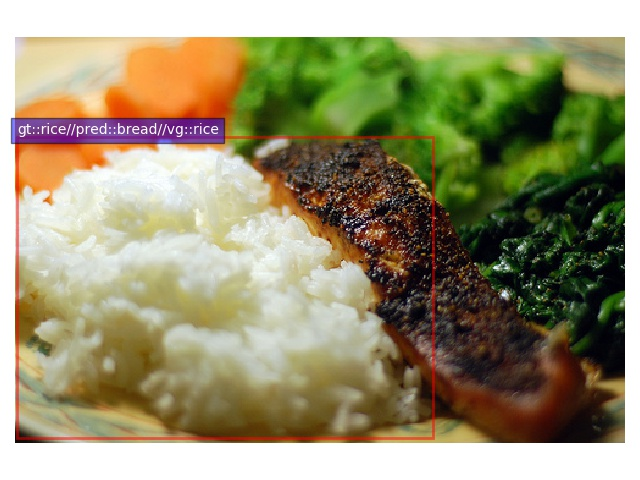
\includegraphics[scale=.2]{images/2323938.jpg}
	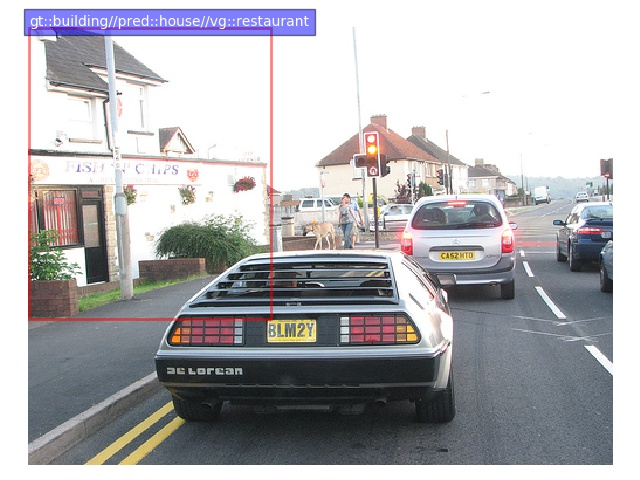
\includegraphics[scale=.2]{images/2322259.jpg}
	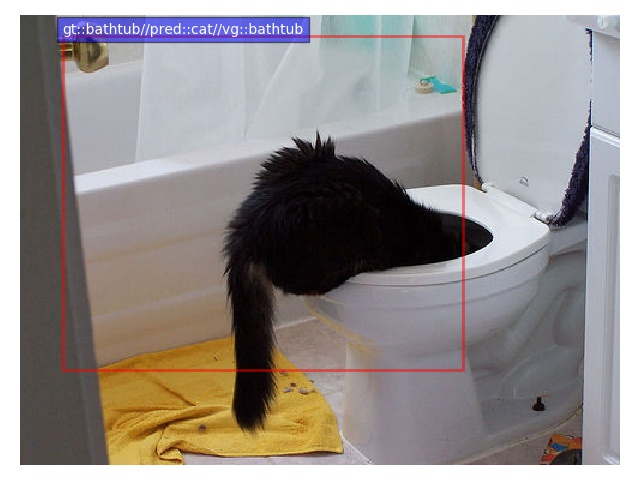
\includegraphics[scale=.2]{images/2371657.jpg}
	
	\caption{TODO: examples resnet mistakes (trained on vg\_manynames, tested on manynames-442)\label{fig:mistakes} \gbt{Will we have space for the figure? (Maybe we should \textit{make} space?) Also, shouldn't we put examples from the most successful model instead?}}
\end{figure}

\cs{TODO::}
Categorization of "errors" (see Figure~\ref{fig:mistakes}):
\begin{enumerate}
	\item Clear mistake \\
	e.g.,\ rice vs. bread
	\item Alternative name\\
	e.g.,\ building vs. house
	\item Alternative object \cs{(other cluster from verif data)}
	\item Synonym\\
	e.g.,\ plane vs. airplane
	\item Semantically related\\
	e.g.,\  motorcycle vs. scooter
\end{enumerate}


\paragraph{Human Object Naming through Transfer-Learning} Figure \ref{fig:exp_confusions} visualizes the change in predictions for  some of our retrained and finetuned models with respect to the object detection baseline (bottom-up-1600). For each object, where the new model predicts a different name than the baseline model, we look at the hit-error categories of the original and new predicted name. Observations:
\begin{itemize}
	\item Retraining faster-rcnn on fewer, entry-level names does not lead to better calibration of entry-level names: more original hits change to same-cluster predictions than the other way round. (top left matrix)
	\item Finetuning the original faster-rcnn on many names recalibrates many decision from same-cluster names to the correct hit. Interestingly, also clear errors are calibrated to perfect hits, whereas hardly any error is changed to same-cluster or related.  (top right matrix)
	\item A similar tendency can be found for the ResNet models: finetuning ResNet on MN changes many predictions from same-cluster to hits. This is less the case when ResNet is finetuned on VG annotations.
	\item Interestingly, both ResNet models change hits into related names (hypernyms, hyponyms, cp-hyponyms) -- why does this happen?
\end{itemize}



\subsection{[TBC] Humans vs. Models: Which Mistakes do they Make?}
\label{sect:exp_analysis}

\paragraph{Categorization of Errors}
see Figure\ ref{fig:mistakes}
\begin{enumerate}
	\item Clear mistake \\
	e.g.,\ rice vs. bread
	\item Alternative name\\
	e.g.,\ building vs. house
	\item Alternative object \cs{(other cluster from verif data)}
	\item Synonym\\
	e.g.,\ plane vs. airplane
	\item Semantically related\\
	e.g.,\  motorcycle vs. scooter
\end{enumerate}

\begin{figure}
	\centering
	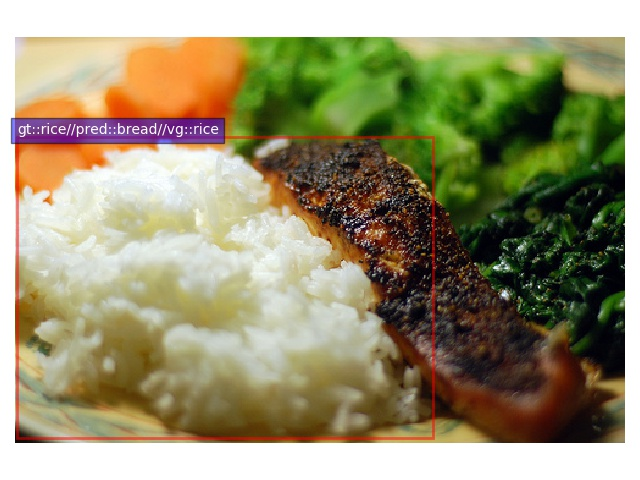
\includegraphics[scale=.2]{images/2323938.jpg}
	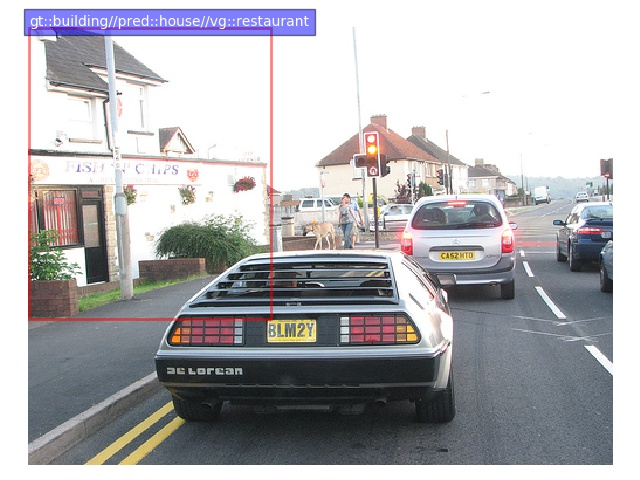
\includegraphics[scale=.2]{images/2322259.jpg}
	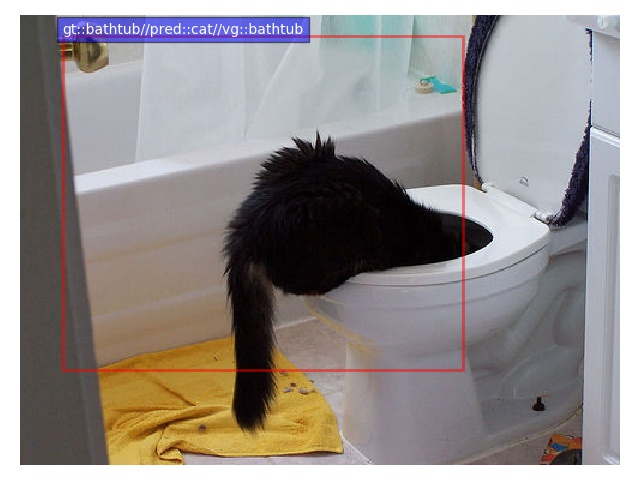
\includegraphics[scale=.2]{images/2371657.jpg}
	
	\caption{resnet mistakes (trained on vg\_manynames, tested on manynames-442)\label{fig:matrices}}
\end{figure}

\subsection{Results}

\paragraph{Overview}
Table\ \ref{tab:exp_overview_results}: \cs{Shows the overview and what MN adds without going into detail: Standard evaluation -- hit; We can additionally distinguish between correct (name alternative, see caption of Table) and clear mistake.}

\paragraph{How do predictions change?} Figure \ref{fig:matrices} visualizes the change in predictions for  some of our retrained and finetuned models with respect to the object detection baseline (bottom-up-1600). For each object, where the new model predicts a different name than the baseline model, we look at the hit-error categories of the original and new predicted name. Observations:
\begin{itemize}
\item Retraining faster-rcnn on less names does not lead to better calibration of entry-level names: more original hits change to same-cluster predictions than the other way round. (top left matrix)
\item Finetuning the original faster-rcnn on many names recalibrates many decision from same-cluster names to the correct hit. Interestingly, also clear errors are calibrated to perfect hits, whereas hardly any error is changed to same-cluster or related.  (top right matrix)
\item A similar tendency can be found for the ResNet models: finetuning ResNet on MN changes many predictions from same-cluster to hits. This is less the case when ResNet is finetuned on VG annotations.
\item Interestingly, both ResNet models change hits into related names (hypernyms, hyponyms, cp-hyponyms) -- why does this happen?
\end{itemize}


\paragraph{Correct predictions}
Table\ \ref{tab:exp_details_correct}: \cs{Gives detailed results to the categories of "correct name" (but not hit): same cluster, WordNet synonym, WordNet hypernym/hyponym}\\
To look into in detail (example images): 
\begin{itemize}
	\item Compare FRCNN vs. FRCNN-finetuned (row block 1 vs. row block 2) with respect to the synonym categories (i.e., predicted name is in a synonym/synonyms\_cluster-relation to the target object) vs. same\_cluster (i.e., predicted name is in response set). 
\end{itemize}

\paragraph{Wrong predictions}

Table\ \ref{tab:exp_details_wrong}: \cs{Gives detailed results to the categories of predicted name\ $\hat{n}$ is incorrect: WordNet co-hyponyms,  other object (inadequacy types: visual, linguistic, bounding box, other (types other+None), $\text{count}(\hat{n})<2$, error (just wrong+unkn(not found in WordNet))}


%%% Local Variables:
%%% mode: latex
%%% TeX-master: "acl2020_main"
%%% End:
